%-*-latex-*-
\sectionthree{Bernoulli trials and Binomial distribution}
\begin{python0}
from solutions import *; clear()
\end{python0}

At this point, we have the basic concept of the probability attached to
a random experiment.
I have also talked about an experiment that is broken up into two
independent random experiment -- this is when the pdf is a product of
two pdfs.

Now I want to talk about the case where
a random experiment involves
performing a \textit{sequence} of the \textit{same} random experiment.
The sequence need not be made up of two experiments.
Usually there's no limit on the size of the sequence.
In fact, I am usually interested in questions like
\lq\lq
How many times do I need to execute this random experiment
until a goal is reached?''

To be specific, consider the following question:

\lq\lq If there's a 32\% chance of making \$1 when I buy
one google stock on Monday at 10:42AM and sell it on the same day at 2:45PM,
what is the chance of me making \$100 if I buy and sell one google
stock according to the above day and times for 200 consecutive
Mondays when the stock market is open''.
Or:
\lq\lq How many consecutive Mondays of trading do I need to execute before
I made 20 days of gains?''


A 
\defterm{Bernoulli trial}
is a random experiment with two outcomes.
This term is used especially when the Bernoulli trials
are performed in a sequence such that the trials are mutually
independent.

For instance suppose I have a biased coin: 
the probability of getting head is 1/3.
What then is the probability of getting 4 heads when the coin 
is tossed 10 times?

Let me put everything into proper mathematical notation.
Let pdf $p_i : S_i \rightarrow [0,1]$
denote the $i$--th time you are tossing the coin.
Note that 
\[
S_i = \{\HEAD, \TAIL\}
\]
and
\[
p_i(\HEAD) = 1/3, \,\,\,\, p_i(\TAIL) = 2/3
\]
(they are all the same, i.s., $S_i = S_j$ and $p_i = p_j$).
The experiments are mutually independent.
Therefore if $p : S \rightarrow [0,1]$ is the pdf
for the experiment of tossing the coin 10 times 
where $S = S_1 \times \cdots \times S_{10}$,
then
\[
p(x_1, \ldots, x_{10}) = p_1(x_1) \cdots p_{10}(x_{10})
\]
(Note that the probability is a product since
the $i$--th toss is independent of the $j$--th toss for $i \neq j$.)
I am interested in the event
\[
A = \{(x_1, \ldots, x_{10}) \in S \mid 
\text{exactly four of the $x_i$'s are $\HEAD$}\}
\]
Note that 
\[
|A| = \binom{10}{4}
\]
and each element of $A$ has the same probability as
the case where the first four tosses are heads:
\begin{align*}
&p(\HEAD, \HEAD, \HEAD, \HEAD, \TAIL, \ldots, \TAIL) \hspace{1cm} \text{(4 heads, 6 tails)}\\
&= p_1(\HEAD) \cdot p_2(\HEAD) \cdot p_3(\HEAD) \cdot p_4(\TAIL) \cdots p_{10}(\TAIL) \\
&= (1/3)^4 (2/3)^4
\end{align*}
Therefore the required probability is
\[
p(A) = \binom{10}{4} (1/3)^4 (2/3)^6 
\]


Because a Bernoulli trial has two outcomes,
it's common to call one of the outcomes a
\defterm{success}\index{success}\index{success \\ failure}
and the other a
\defterm{failure}\index{failure}.

In general, you see right away that:

\begin{thm}
If the probability of the success of a Bernoulli trial is $p$,
then the probability of having $k$ successes when performing
$n$ of the Bernoulli trials is given by 
\[
\binom{n}{k} p^k (1-p)^{n-k}
\]
\qed
\end{thm}

Frequently you will see the following notations:
\[
B_{n,p}(k) = \binom{n}{k} p^k (1-p)^{n-k}
\]
Other notations include
\[
B(n,p; k)
\text{ \,\,\, and \,\,\, }
B(n,p,k)
\]

Frequently the $n$ and $p$ are fixed and $k$ is considered the
variable of the pdf $B(n,p)$.

Formally, define the pdf of a \defone{Bernoulli trial} as
\[
p_{\textsc{Bernoulli}}: \{\textsc{Success}, \textsc{Failure}\} \rightarrow [0, 1]
\]
Instead of using the outcomes \textsc{Success}
and \textsc{Failure}, it's useful to label them as $1$ and $0$.
In other words, it's useful to have a Bernoulli trial random variable
defined as
\[
X_{\textsc{Bernoulli}} : \{\textsc{Success}, \textsc{Failure}\} \rightarrow \{1, 0\}
\]
where
\[
X_{\textsc{Bernoulli}}(\textsc{Success}) = 1, \,\,\,\,\,
X_{\textsc{Bernoulli}}(\textsc{Failure}) = 0
\]
especially since for the corresponding Binomial distribution I'll
need to count the number of successes.
In other words $X_{\textsc{Bernoulli}}$
is an indicator random variable of \textsc{Success}.
All the above notations are for a single Bernoulli trial.
Now we define the \defone{Binomial distribution}.

Associated with a given Bernoulli trial
$p_{\textsc{Bernoulli}}$, 
we define the $n$--fold product pdf,
the \defone{Binomial distribution} 
\[
p_{B(n,p)}:
\{\textsc{Success}, \textsc{Failure}\}^n \rightarrow [0, 1]
\]
as
\[
p_{B(n,p)}(x_0, x_1, \ldots, x_{n - 1}) =
p_0(x_0) \cdots p_{n-1}(x_{n-1})
\]
where $p_i$ is the pdf of the $i$--th Bernoulli trial
where the \lq\lq $p$" is the probability of success of
the Bernoulli trail.
Of course $p_i = p_{\textsc{Bernoulli}}$, i.e.,
\[
p_{B(n,p)}(x_0, x_1, \ldots, x_{n - 1}) =
p_{\textsc{Bernoulli}}(x_0) \cdots p_{\textsc{Bernoulli}}(x_{n-1})
\]
Let $X_i$ be the indicator random variable for a success
for the $i$--th Bernoulli trial, i.e.,
\[
X_i(x_0, ..., x_{n-1})
=
\begin{cases}
  1 & \text{ if } x_i = \textsc{Success}\\
  0 & \text{ otherwise}\\
\end{cases}
\]
In other words
\[
X_i(x_0, ..., x_{n-1}) = X_{\textsc{Bernoulli}}(x_i)
\]
Next define the random variable
\[
X_{B(n,p)} = \sum_{i=0}^{n-1} X_i
\]
Then
\[
B_{n,p}(k) = \Pr[X_{B(n,p)} = k]
\]
With these notation, the above theorem says
\[
B_{n,p}(k) = \Pr[X_{B(n,p)} = k] = \binom{n}{k} p^k (1 - p)^{n-k}
\]

Here's a plot of $B_{30, 1/10}$:
\begin{center}
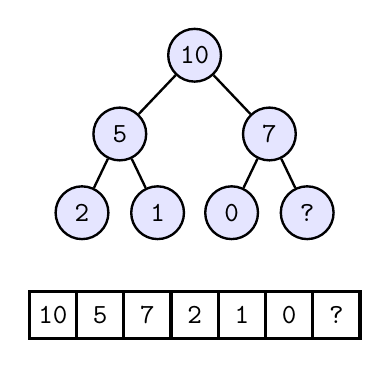
\begin{tikzpicture}

\fill[blue!10] (0.0, 0.0) circle (0.35);
\node [line width=0.03cm,black,minimum size=0.6699999999999999cm,draw,circle] at (0.0,0.0)(10){};\draw (0.0, 0.0) node[color=black] {\texttt{10}};
\fill[blue!10] (-0.95, -1.0) circle (0.35);
\node [line width=0.03cm,black,minimum size=0.6699999999999999cm,draw,circle] at (-0.95,-1.0)(5){};\draw (-0.95, -1.0) node[color=black] {\texttt{5}};
\fill[blue!10] (0.95, -1.0) circle (0.35);
\node [line width=0.03cm,black,minimum size=0.6699999999999999cm,draw,circle] at (0.95,-1.0)(7){};\draw (0.95, -1.0) node[color=black] {\texttt{7}};
\fill[blue!10] (-1.43, -2.0) circle (0.35);
\node [line width=0.03cm,black,minimum size=0.6699999999999999cm,draw,circle] at (-1.43,-2.0)(2){};\draw (-1.43, -2.0) node[color=black] {\texttt{2}};
\fill[blue!10] (-0.47, -2.0) circle (0.35);
\node [line width=0.03cm,black,minimum size=0.6699999999999999cm,draw,circle] at (-0.47,-2.0)(1){};\draw (-0.47, -2.0) node[color=black] {\texttt{1}};
\fill[blue!10] (0.47, -2.0) circle (0.35);
\node [line width=0.03cm,black,minimum size=0.6699999999999999cm,draw,circle] at (0.47,-2.0)(0){};\draw (0.47, -2.0) node[color=black] {\texttt{0}};
\fill[blue!10] (1.43, -2.0) circle (0.35);
\node [line width=0.03cm,black,minimum size=0.6699999999999999cm,draw,circle] at (1.43,-2.0)(?){};\draw (1.43, -2.0) node[color=black] {\texttt{?}};\draw[line width=0.03cm,black] (10) to  (5);
\draw[line width=0.03cm,black] (10) to  (7);
\draw[line width=0.03cm,black] (5) to  (2);
\draw[line width=0.03cm,black] (5) to  (1);
\draw[line width=0.03cm,black] (7) to  (0);
\draw[line width=0.03cm,black] (7) to  (?);

\draw (-1.8, -3.3)
  node[draw, line width=0.04cm, , color=black,
       rounded corners=0cm, inner sep=0cm] {

\begin{minipage}[t][0.6cm]{0.6cm}
\mbox{}

\end{minipage}

};\draw (-1.8, -3.3) node[color=black] {{\texttt{10}}};
\draw (-1.2, -3.3)
  node[draw, line width=0.04cm, , color=black,
       rounded corners=0cm, inner sep=0cm] {

\begin{minipage}[t][0.6cm]{0.6cm}
\mbox{}

\end{minipage}

};\draw (-1.2, -3.3) node[color=black] {{\texttt{5}}};
\draw (-0.6000000000000001, -3.3)
  node[draw, line width=0.04cm, , color=black,
       rounded corners=0cm, inner sep=0cm] {

\begin{minipage}[t][0.6cm]{0.6cm}
\mbox{}

\end{minipage}

};\draw (-0.6000000000000001, -3.3) node[color=black] {{\texttt{7}}};
\draw (-1.1102230246251565e-16, -3.3)
  node[draw, line width=0.04cm, , color=black,
       rounded corners=0cm, inner sep=0cm] {

\begin{minipage}[t][0.6cm]{0.6cm}
\mbox{}

\end{minipage}

};\draw (-1.1102230246251565e-16, -3.3) node[color=black] {{\texttt{2}}};
\draw (0.6, -3.3)
  node[draw, line width=0.04cm, , color=black,
       rounded corners=0cm, inner sep=0cm] {

\begin{minipage}[t][0.6cm]{0.6cm}
\mbox{}

\end{minipage}

};\draw (0.6, -3.3) node[color=black] {{\texttt{1}}};
\draw (1.2, -3.3)
  node[draw, line width=0.04cm, , color=black,
       rounded corners=0cm, inner sep=0cm] {

\begin{minipage}[t][0.6cm]{0.6cm}
\mbox{}

\end{minipage}

};\draw (1.2, -3.3) node[color=black] {{\texttt{0}}};
\draw (1.8, -3.3)
  node[draw, line width=0.04cm, , color=black,
       rounded corners=0cm, inner sep=0cm] {

\begin{minipage}[t][0.6cm]{0.6cm}
\mbox{}

\end{minipage}

};\draw (1.8, -3.3) node[color=black] {{\texttt{?}}};
\end{tikzpicture}

\end{center}


and here's a plot of $B_{30, 5/6}$::
\begin{center}
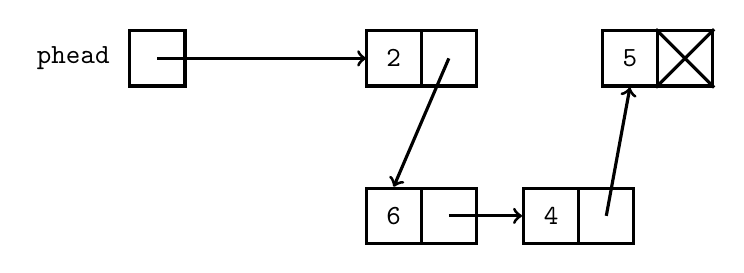
\begin{tikzpicture}

\draw (0.35, 0.35)
  node[draw, line width=0.04cm, , color=black,
       rounded corners=0cm, inner sep=0cm] {

\begin{minipage}[t][0.7cm]{0.7cm}
\mbox{}

\end{minipage}

};\draw (0.35, 0.35) node[color=black] {{\texttt{2}}};
\draw (1.0499999999999998, 0.35)
  node[draw, line width=0.04cm, , color=black,
       rounded corners=0cm, inner sep=0cm] {

\begin{minipage}[t][0.7cm]{0.7cm}
\mbox{}

\end{minipage}

};\draw (1.0499999999999998, 0.35) node[color=black] {{\texttt{}}};
\draw (0.35, -1.65)
  node[draw, line width=0.04cm, , color=black,
       rounded corners=0cm, inner sep=0cm] {

\begin{minipage}[t][0.7cm]{0.7cm}
\mbox{}

\end{minipage}

};\draw (0.35, -1.65) node[color=black] {{\texttt{6}}};
\draw (1.0499999999999998, -1.65)
  node[draw, line width=0.04cm, , color=black,
       rounded corners=0cm, inner sep=0cm] {

\begin{minipage}[t][0.7cm]{0.7cm}
\mbox{}

\end{minipage}

};\draw (1.0499999999999998, -1.65) node[color=black] {{\texttt{}}};
\draw (2.35, -1.65)
  node[draw, line width=0.04cm, , color=black,
       rounded corners=0cm, inner sep=0cm] {

\begin{minipage}[t][0.7cm]{0.7cm}
\mbox{}

\end{minipage}

};\draw (2.35, -1.65) node[color=black] {{\texttt{4}}};
\draw (3.0500000000000003, -1.65)
  node[draw, line width=0.04cm, , color=black,
       rounded corners=0cm, inner sep=0cm] {

\begin{minipage}[t][0.7cm]{0.7cm}
\mbox{}

\end{minipage}

};\draw (3.0500000000000003, -1.65) node[color=black] {{\texttt{}}};
\draw (3.35, 0.35)
  node[draw, line width=0.04cm, , color=black,
       rounded corners=0cm, inner sep=0cm] {

\begin{minipage}[t][0.7cm]{0.7cm}
\mbox{}

\end{minipage}

};\draw (3.35, 0.35) node[color=black] {{\texttt{5}}};
\draw (4.05, 0.35)
  node[draw, line width=0.04cm, , color=black,
       rounded corners=0cm, inner sep=0cm] {

\begin{minipage}[t][0.7cm]{0.7cm}
\mbox{}

\end{minipage}

};\draw (4.05, 0.35) node[color=black] {{\texttt{}}};\draw[line width=0.04cm,black,->] (1.05,0.35) to  (0.35,-1.28);
\draw[line width=0.04cm,black,->] (1.05,-1.65) to  (1.98,-1.65);
\draw[line width=0.04cm,black,->] (3.05,-1.65) to  (3.35,-0.02);
\draw[line width=0.04cm,black] (3.68,0.72) to  (4.42,-0.02);
\draw[line width=0.04cm,black] (4.42,0.72) to  (3.68,-0.02);

\draw (-2.65, 0.35)
  node[draw, line width=0.04cm, , color=black,
       rounded corners=0cm, inner sep=0cm] {

\begin{minipage}[t][0.7cm]{0.7cm}
\mbox{}

\end{minipage}

};\draw (-2.65, 0.35) node[color=black] {{\texttt{}}};\draw[line width=0.04cm,black,->] (-2.65,0.35) to  (0,0.35);

\draw (-3.7199999999999998, 0.35)
  node[draw, line width=0.04cm, , color=white,
       rounded corners=0cm, inner sep=0cm] {

\begin{minipage}[t][0.1cm]{0.1cm}
\mbox{}

\end{minipage}

};\draw (-3.7199999999999998, 0.35) node[color=black] {{\texttt{phead}}};
\end{tikzpicture}

\end{center}



\newpage
%-*-latex-*-

\begin{ex} 
  \label{ex:prob-00}
  \tinysidebar{\debug{exercises/{disc-prob-28/question.tex}}}

  \solutionlink{sol:prob-00}
  \qed
\end{ex} 
\begin{python0}
from solutions import *
add(label="ex:prob-00",
    srcfilename='exercises/discrete-probability/prob-00/answer.tex') 
\end{python0}

%-*-latex-*-

\begin{ex} 
  \label{ex:prob-00}
  \tinysidebar{\debug{exercises/{disc-prob-28/question.tex}}}

  \solutionlink{sol:prob-00}
  \qed
\end{ex} 
\begin{python0}
from solutions import *
add(label="ex:prob-00",
    srcfilename='exercises/discrete-probability/prob-00/answer.tex') 
\end{python0}

%-*-latex-*-

\begin{ex} 
  \label{ex:prob-00}
  \tinysidebar{\debug{exercises/{disc-prob-28/question.tex}}}

  \solutionlink{sol:prob-00}
  \qed
\end{ex} 
\begin{python0}
from solutions import *
add(label="ex:prob-00",
    srcfilename='exercises/discrete-probability/prob-00/answer.tex') 
\end{python0}

%-*-latex-*-

\begin{ex} 
  \label{ex:prob-00}
  \tinysidebar{\debug{exercises/{disc-prob-28/question.tex}}}

  \solutionlink{sol:prob-00}
  \qed
\end{ex} 
\begin{python0}
from solutions import *
add(label="ex:prob-00",
    srcfilename='exercises/discrete-probability/prob-00/answer.tex') 
\end{python0}

%-*-latex-*-

\begin{ex} 
  \label{ex:prob-00}
  \tinysidebar{\debug{exercises/{disc-prob-28/question.tex}}}

  \solutionlink{sol:prob-00}
  \qed
\end{ex} 
\begin{python0}
from solutions import *
add(label="ex:prob-00",
    srcfilename='exercises/discrete-probability/prob-00/answer.tex') 
\end{python0}

%-*-latex-*-

\begin{ex} 
  \label{ex:prob-00}
  \tinysidebar{\debug{exercises/{disc-prob-28/question.tex}}}

  \solutionlink{sol:prob-00}
  \qed
\end{ex} 
\begin{python0}
from solutions import *
add(label="ex:prob-00",
    srcfilename='exercises/discrete-probability/prob-00/answer.tex') 
\end{python0}


